\documentclass[11pt,letterpaper]{article}
\usepackage[margin=0.85in]{geometry}
\usepackage{amsmath,amssymb,booktabs,array,longtable,graphicx}
\usepackage{xcolor}
\usepackage{enumitem}
\usepackage{fancyhdr}
\usepackage{hyperref}
\hypersetup{colorlinks=true,linkcolor=blue!45!black,urlcolor=blue!45!black,
  citecolor=blue!45!black,pdftitle={Ember: status and the path to complete low-mass stellar lifetimes},
  pdfauthor={Ember project, prepared for Gregory Laughlin}}
\definecolor{ember}{HTML}{A4492A}
\setlength{\parindent}{0pt}
\setlength{\parskip}{6pt}
\setlength{\emergencystretch}{2em}
\setlist{nosep,leftmargin=*}
\pagestyle{fancy}
\fancyhf{}
\fancyhead[L]{\small\textcolor{ember}{EMBER}\quad Scientific checkpoint}
\fancyhead[R]{\small 9 September 2026}
\fancyfoot[C]{\small\thepage}
\setlength{\headheight}{14pt}
\newcommand{\Ms}{M_\odot}
\newcommand{\Rs}{R_\odot}
\newcommand{\Ls}{L_\odot}
\newcommand{\Tyr}{\mathrm{Tyr}}
\newcommand{\doc}[2]{\href{https://github.com/oklo/ember/blob/master/#1}{#2}}

\begin{document}
\begin{center}
{\LARGE\bfseries\textcolor{ember}{Ember}}\\[6pt]
{\Large Status and the path to complete\\low-mass stellar lifetimes}\\[8pt]
{\normalsize Scientific and operational handoff for Gregory Laughlin}\\[3pt]
{\small Physics snapshot: 9 September 2026, 23:09 UTC}
\end{center}

\textbf{Principal result.} A fixed-baryonic-mass $0.1\Ms$ model has reached
$2.85\times10^{12}$ yr with composition-dependent microphysics and a non-grey
gas atmosphere. It remains fully convective and retains $X_{\rm H}=0.30289$.
This is a reproducible partial hydrogen-burning track, \emph{not} a measured
stellar lifetime, a completed blue-dwarf excursion, or a white-dwarf cooling
calculation. Here $1\Tyr=10^{12}$ yr.

The current input-development bottlenecks are atmospheric coverage below
$X_{\rm H}=0.3$, independently validated hydrogen-poor opacity interpolation,
and condensate thermodynamics in layers carrying a small convective flux.
The new hydrogen-poor EOS is available separately, but neither it nor the
new opacity family is selected by the reference trajectory. Condensate
feedback is absent from that trajectory.

\textbf{Distribution.} GitHub carries code, generation specifications, small
provenance records and this report. New bulk physics tables, raw histories,
source-output archives and checkpoint binaries remain local. The committed
generation pipeline is described in \doc{docs/DATA_REPRODUCTION.md}{DATA\_REPRODUCTION.md}.

\section{The current $0.1\Ms$ model}
The initial state is a specified static main-sequence model with
$X_{\rm H}=0.7$, $X_3=0$, $Z=0.02$, and the GS98 metal pattern.
Its age excludes formation and pre-main-sequence contraction. All abundances
below use conserved baryonic mass. Values are reported to identify the model;
the displayed digits do not represent physical accuracy.

\begin{center}
\begin{tabular}{@{}lr@{}}
\toprule
Quantity & Last completed model \\
\midrule
Age from the static initial model & $2.85\Tyr$ \\
Mass used in the structure equations & $0.1\Ms$ \\
Radius & $0.148760882\Rs$ \\
Surface luminosity & $0.00185757060\Ls$ \\
Effective temperature & $3106.8375$ K \\
Central temperature & $6.878544$ MK \\
Central density & $241.23194\ \mathrm{g\,cm^{-3}}$ \\
Central pressure & $1.6524980\times10^{17}\ \mathrm{dyn\,cm^{-2}}$ \\
Surface $\log_{10}g$ (cgs) & $5.0930901$ \\
$X_{\rm H},\ X_3,\ X_4$ & $0.302887598,\ 0.004663338,\ 0.672449064$ \\
Metal mass fraction & $0.02$ \\
Convective mass fraction & $1$ (homogeneous) \\
Mesh; accepted/rejected macrosteps & $512$; $1673/1$ \\
\bottomrule
\end{tabular}
\end{center}

The minimum midpoint ratio of the gradient required for entirely diffusive
transport to the adiabatic gradient is $3.19869$. The largest estimated local
conductive flux fraction is $0.0328883$; the central value is $0.0086111$.
The maximum reduced ppII/pp reaction ratio is $0.00296634$.
These are diagnostics of this model, not guarantees about subsequent evolution.
The records are the evolution, transport and nuclear
\doc{docs/results/evolution_metal_m010_2850gyr_gas.json}{2.85T reports}.

\section{What has been built}
Ember is a C++23 reconstruction and extension of the stellar-evolution line
recovered in the historical \href{https://github.com/oklo/Henyey}{Henyey/F77}
repository. LBA97 supplies the scientific benchmark and evolutionary picture
\cite{lba97}; it does not supply a lifetime that the new calculation is required
to reproduce. The developments below describe Ember's present implementation,
rather than asserting that the older code lacked every underlying physical effect.

\begin{longtable}{@{}>{\raggedright\arraybackslash}p{0.19\textwidth}p{0.75\textwidth}@{}}
\toprule
Component & Implemented treatment and qualification \\
\midrule
\endhead
Equation of state & FreeEOS 3.0 EOS1 represented by one interpolated Helmholtz
potential, with consistent caloric and response derivatives. Molecular formation,
ionization, pressure ionization, electron degeneracy and source nonideal terms
are included within supported states. The current family includes GS98 metals
and explicit H/He3 composition dependence. Potassium, with mass fraction
$4.56\times10^{-6}$, is omitted by this source. Helium isotope corrections retain
electronic/cross-section approximations. \\[5pt]
Radiative opacity & Composition-dependent AESOPUS 2.1 low-temperature gas opacity
and LANL TOPS hot/dense opacity, with supported blends and isotope number-density
mapping. The existing interior families cover $Z=.01,.02,.03$; this is a modest
interval, not a high-metallicity survey. Substituted source cells and extrapolation
are rejected. \\[5pt]
Nuclear burning & Explicit non-equilibrium $^3$He, reduced ppI/ppII burning,
Solar Fusion II S-factor quadrature, finite-degeneracy Salpeter--Van Horn
screening, nuclear-neutrino losses and heating derived consistently from atomic
mass defects. No pep, hep, ppIII or CNO network; the reduced ppII completion and
neutrino approximation are documented. \\[5pt]
Transport & MLT with Schwarzschild or full-EOS Ledoux buoyancy. Electron
conduction uses Ioffe/Cassisi-family inputs and approximate mixture resistivities.
Slow semiconvective and thermohaline composition mixing are available. The
semiconvective option has no separate heat flux. No microscopic settling. \\[5pt]
Atmosphere & Offline TLUSTY208/SYNSPEC54 LTE, plane-parallel radiative/convective
gas models, matched at $\tau=100$. Molecular and atomic opacity, collision-induced
absorption and scattering are included. Runtime interpolation is in H, He3,
$T_{\rm eff}$ and gravity. The installed extension has 72 source cells. \\[5pt]
Evolution and checks & Analytic zone Jacobians; damped Henyey/Newton structure
solution; coupled implicit burning and conservative mixing; the discrete thermal
first law; adaptive timestep control by step doubling. Fixed mass mesh.
Native checkpoints preserve internal state and timestep-controller state;
source and executable fingerprints protect reproducibility. \\
\bottomrule
\end{longtable}

Physical consistency still has identifiable limits. The EOS, atmosphere chemistry,
line/continuum opacities and conduction do not all come from one common
thermodynamic source. At matching states of the extended gas grid, interior-EOS
densities differ from atmospheric-EOS densities by approximately $0.68$--$1.99\%$.
The common metal inventory improves agreement without removing atomic-weight,
partition-function and isotope approximations. Nuclear screening is not derived
from the FreeEOS interaction free energy. The conduction mixture uses approximate
addition of pure-ion collision effects, and its envelope activation is an explicit
domain join rather than a partial-ionization conductivity calculation.

\section{The track and the evidence for numerical reliability}
\begin{figure}[ht]
\centering
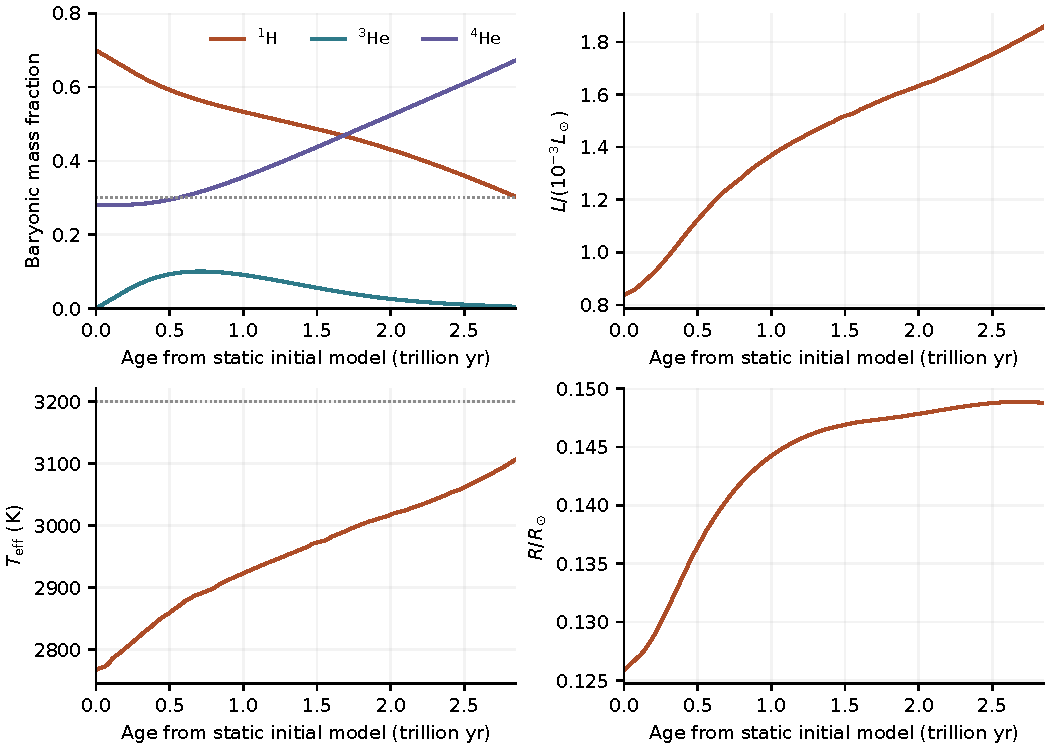
\includegraphics[width=\textwidth]{evolution_history.pdf}
\caption{The completed gas-atmosphere trajectory, assembled from the original
0--2.5T run and the 2.5--2.75T and 2.75--2.85T native continuations. The 1674
recorded states include the initial state and 1673 accepted macrosteps. Duplicate
restart rows are removed only after equality checks on the overlapping physical
states. Dotted lines show the present atmospheric H floor (upper left) and
effective-temperature ceiling (lower left). The late, small radius turnover
has not been established by late-time numerical refinement.}
\end{figure}

The star first builds a substantial non-equilibrium $^3$He reservoir and later
consumes it. A continuation-only maximum must not be reported as the maximum
over the entire history. The evolving luminosity, abundance and surface temperature
show why a fixed-composition boundary is insufficient for a multi-trillion-year
calculation.

\begin{center}
\begin{tabular}{@{}lrr@{}}
\toprule
Same-physics comparison at 2T & $\Delta L/L$ & $\Delta R/R$ \\
\midrule
512 $\rightarrow$ 1024 mesh points & $+0.061632\%$ & $-0.012340\%$ \\
Fourfold tighter time tolerances & $-0.003610\%$ & $-0.000594\%$ \\
\bottomrule
\end{tabular}
\end{center}
An independent complete 2T run reproduces the history and profile byte for byte.
The checkpoint-enabled executable also reproduces the original 2.5T output
exactly. Native restart tests compare subsequent accepted histories and final
profiles, including executable relocation and rejection of incompatible inputs.
The last 2.75--2.85T continuation took 37 accepted steps and no rejections.

These establish repeatability and numerical sensitivity of the completed
segments. They do not establish lifetime convergence, a universal error bound,
or physical accuracy of the sources. The energy-balance diagnostics check the
implemented discrete first law; they are not an independent proof of an exact
global gravitational-energy balance.

\section{Input development: accepted, diagnostic, and blocked work}
\subsection{Hydrogen-poor EOS: available, not selected}
A separate GS98 $Z=.02$ family now contains 24 planes:
$X_{\rm H}=.1,.125,.15,.175,.2,.25,.3,.4,.5,.6,.7,.75$ at
$X_3=0,.12$. All original $X_{\rm H}\geq.3$ planes are retained byte for byte.
A coarser composition spacing produced a $1.22\%$ heat-capacity discrepancy,
so extra planes were computed before acceptance. Across 336 fresh source
comparisons, maximum discrepancies are $0.04985\%$ in pressure,
$0.10866\%$ in energy and $0.19344\%$ in heat capacity. First-law/response
checks are below $7.2\times10^{-10}$. All 1536 sampled states from the 2T,
2.5T and 2.75T profiles give byte-identical old/new EOS probe output.
The scope and source manifests are in
\doc{docs/FORWARD_EVOLUTION.md}{FORWARD\_EVOLUTION.md}.

\subsection{Hydrogen-poor opacity: under validation}
The separate TOPS extension has 30 planes, covering source H fractions
$.09,.1,.2,.3,.4,.5,.6,.65,.7,.75$ at $Z=.01,.02,.03$.
The extra $.09$ plane brackets the atomic/source composition corresponding to
baryonic $X_{\rm H}=.1$ with $X_3=.12$. Original planes and old-profile evaluations
are unchanged; support and derivative checks pass.

\textbf{An independent midpoint source exposed a real interpolation limitation.}
At $X=.15,Z=.02$, comparison against the $.1/.2$ interpolation over 3496
common original source cells, excluding 54 substituted cells, gives a maximum
discrepancy of $11.9011\%$. The worst discrepancy within the audit's defined hot
rectangle is $0.918319\%$. The all-cell maximum is not a measured error in the
current star: the active blend and sampled stellar states must be considered.
Neither result is a physical uncertainty estimate for TOPS itself.

Four further source fetches completed: $X=.15$ at $Z=.01,.03$ and independent
quarter-points $X=.125,.175$ at $Z=.02$. This handoff archives their raw requests
and results without importing or accepting a refined runtime family. Rounded
filenames \texttt{x012/x018} must not be interpreted as actual $.12/.18$ mixtures.
The original midpoint audit must survive any promotion of that midpoint to a
new interpolation node.

\subsection{Atmosphere and condensates: the current physical block}
The installed gas family spans $X_{\rm H}=.3,.45,.7$, $X_3=0,.12$,
$T_{\rm eff}=2600,2800,3000,3200$ K and $\log g=4.9,5.15,5.4$.
A separate heldout gas atmosphere gives local interpolation differences of
$0.19584\%$ in temperature and $0.03401\%$ in gas pressure at the matching point.
The corresponding deeper material-temperature coverage is approximately
1076--7762 K. A proposed extension to 15000 K encountered unsupported native
He I 4471 broadening; clipping or extrapolation has not been substituted for
valid source coverage.

FastChem equilibrium/rainout diagnostics and coupled gas-depletion experiments
have been built. The coupled experiment is an efficient-settling limit with
\emph{zero grain opacity}, hybrid depletion/gas chemistry, and no grain
enthalpy, size distribution, Mie opacity or time-dependent settling.
The last collector accepted 70 of 72 proposed production cells. Both remaining
solar 2800 K, $\log g=4.9$ corners now have converged solutions but fail the
physical grain-enthalpy gate: convective flux fractions in condensing layers are
approximately $4.17\times10^{-7}$ ($X_3=.12$) and $4.11\times10^{-7}$ ($X_3=0$),
above the unchanged $10^{-8}$ threshold. Moving to $\log g=5.0$ did not remove
the problem.

Artificial positive heat-capacity perturbations of $10^6$ and
$10^7\ \mathrm{erg\,g^{-1}\,K^{-1}}$ at an actual failing corner have completed.
They change the matching gas pressure by $7.49\times10^{-7}$ and
$7.38\times10^{-6}$ fractionally, respectively. They are useful sensitivity
controls, not a full grain EOS or a rigorous bound on missing physics.
There is no installed condensate runtime family or install receipt.

\section{Physical requirements along the remaining evolution}
The expected isolated-star path is prolonged helium enrichment, a hotter
excursion, a radiative/conductive core, central H exhaustion, residual shell
burning and a helium-remnant cooling sequence \cite{lba97,adams97}.
Each stage changes the applicability of current approximations.

\subsection{Radiative-core formation and redistribution of fuel}
Once full convection ends, microscopic gravitational settling and thermal/chemical
diffusion can compete with burning and boundary motion. Their timescales need
evaluation over the actual density, temperature and composition profiles.
Resolving moving convection boundaries, steep composition gradients and thin
shells may require adaptive remeshing. Semiconvective heat transport and the
sensitivity to mixing efficiencies also need attention. These are acknowledged
roadmap tasks; the implemented Ledoux/mixing tests do not yet demonstrate the
evolved stellar transition.

\subsection{Exhaustion and residual shell burning}
All input families eventually need support approaching zero H, including
nearly hydrogen-free core material adjacent to a fuel-bearing shell. The reduced
ppII completion assumption needs reassessment when protons become scarce.
The missing pep and other pp branches, CNO catalysts at higher temperature or
metallicity, and screening/EOS consistency require quantitative error assessment.
The nuclear module currently limits its S-factor expansion to $T\leq20$ MK and
rejects quantum-dominated screening states.

Central H exhaustion, cessation of sustained H burning and a later cooling
luminosity must be separate measured endpoints. A residual envelope can remain
energetically relevant after central exhaustion. Diffusion alters residual
burning in helium-white-dwarf calculations \cite{althaus09}; some binary-formed
objects experience unstable CNO shell flashes \cite{istrate14}. These identify
mechanisms to test, not envelope masses or flash thresholds to transplant into
an isolated $0.1\Ms$ star. A flash is not presumed for this reference case.

\subsection{The atmosphere of the emerging remnant}
A helium-rich interior does not determine the photospheric composition.
Residual hydrogen can float upward; later convection can dilute or mix it into
helium-rich material. White-dwarf transport calculations demonstrate both
processes \cite{bedard23}. A future boundary treatment must therefore follow
the resolved surface composition and envelope history.

Cooling brings the object back into cold-atmosphere regimes at different
gravity and density. Relevant inputs include nonideal H/He chemistry,
pressure-distorted collision-induced absorption, dense-fluid continuum opacity,
line broadening and possibly refraction \cite{blouin18}. The current dwarf
atmosphere grid and its condensate experiment do not establish this coverage.
Remnant-envelope transport and dense cool atmospheres lack an operational
implementation plan beyond the broader source-extension goals.

\subsection{Cold ion thermodynamics and remnant cooling}
Electron degeneracy and thermal/gravothermal evolution already exist in Ember.
Further cooling requires appropriate strongly coupled ion thermodynamics,
crystallization and latent heat where applicable, mixture separation, ionic
quantum corrections to heat capacity, and conductivity through the relevant
liquid, solid and partially ionized regimes. Quantum effects can modify the
liquid heat capacity before freezing \cite{baiko19}.

A helium remnant requires its own density- and composition-appropriate phase
physics. Carbon--oxygen phase separation or a standard $^{22}$Ne sedimentation
prescription must not be assigned automatically to a star that never underwent
helium burning. Dense-ion and solid terms are anticipated by the architecture,
but those hooks are not implemented cooling physics.

Full thermal-neutrino losses remain absent from the stellar energy equation.
At 2.85T a plasmon-only post-processing estimate gives
$L_{\nu,\mathrm{plasma}}/L=1.45\times10^{-8}$; it does not evaluate all thermal
channels or establish insignificance throughout later contraction. Their
importance must be checked rather than inferred from present-day conditions.

\section{Effects outside the immediate grid programme}
\subsection{Mass, rotation and magnetic history}
The reference star has fixed baryonic mass and no wind, angular-momentum,
magnetic-convection or starspot evolution. Even weak time-averaged mass loss
can accumulate over trillions of years. For scale only,
\[
 \langle |\dot M|\rangle=10^{-15}\Ms\,\mathrm{yr}^{-1},\qquad
 \Delta t=5\times10^{12}\ \mathrm{yr}
 \quad\Longrightarrow\quad \Delta M=0.005\Ms.
\]
This is 5\% of the reference mass; it is not a prediction that such a wind
persists. The relevant task is to bound the integrated loss under plausible
rotation and magnetic histories, rather than extrapolate a present-day rate
unchanged. These are presently controlled omissions without implemented models.

The integrated nuclear rest-mass release by 2.85T is $0.00282709$ of baryonic
mass. Heating accounts for that release, but Newtonian gravity still uses
conserved baryonic mass. This approximation needs assessment before a precise
cross-code lifetime comparison; mesh refinement cannot remove it.

\subsection{A mass--composition survey includes different branches}
The initial driver, detailed EOS and atmosphere currently target one mass and
$Z=.02$. Helium enrichment by H burning at fixed $Z$ is distinct from a grid
of stars born at high $Z$. The fundamental survey is in mass, initial H/He
abundances and metal pattern. A lifetime$(M,Z)$ curve selects a relation $Y(Z)$
and relative metal abundances. Independent high-$Z$ EOS/opacity validation is
essential; source availability is not proof of accuracy.

Near the minimum hydrogen-burning mass, initial entropy and contraction must
be tested to distinguish a stable star from a cooling substellar object.
At larger masses, early radiative regions, shell-driven giant expansion and,
if the chosen mass/composition permits, helium ignition require additional
coverage and physics. Repeated $^3$He-driven convective episodes near the
fully convective boundary are a further transport-resolution test
\cite{vansaders12}. They are not missing $^3$He chemistry in the present network.
No giant phase, helium flash or carbon--oxygen remnant is presumed for the
isolated $0.1\Ms$ case.

The metallicity-dependent lifetime maximum discussed by Adams and Laughlin
\cite{adams97} is a hypothesis to bracket numerically. Its location and even
the relevant survey cut depend on helium enrichment, metal pattern and mass.
Neither a specific maximum nor the historical roadmap's nominal 12T duration
is imposed as an answer.

\subsection{The much more remote future}
Encounters, mergers, accretion and the evolving radiation environment require
an environmental model. Possible dark-matter heating requires explicit particle
and halo assumptions. Cold pycnonuclear processing lies outside the current
thermal network, which switches burning off below $10^5$ K. Hypothetical proton
decay adds a different energy, mass and composition evolution problem. Such
conditional extensions belong to a later future-universe programme
\cite{adams97}; none is required to claim an isolated-star hydrogen-burning
lifetime once its stated physical assumptions have been tested.

\section{Priorities and completion criteria}
\begin{enumerate}[label=\textbf{\arabic*.},itemsep=5pt]
\item \textbf{Preserve the reference and finish source validation.} Retain the
accepted gas inputs and failed controls. Compare the completed TOPS refinement
sources on the relevant opacity/blend domain with independent compositions;
publish a separate validated family. Resolve grain enthalpy/convection or
justify a physically controlled alternative before altering production policy.
\item \textbf{Provide the next atmospheric coverage.} Extend H, temperature
and gravity along the star's actual path; independently validate interpolation
and source support. Add explicit input selection. Avoid repeatedly calculating
irrelevant corners solely to fill a large rectangular grid.
\item \textbf{Follow the structural transition.} Compare diffusion, nuclear
and transport timescales; implement significant missing physics. Resolve core
and shell boundaries and demonstrate spatial/timestep convergence there.
Preserve conservative abundance and energy accounting.
\item \textbf{Measure and converge lifetimes.} Record central exhaustion and
the end of sustained burning separately. Vary endpoint thresholds, mesh,
timestep, source-grid resolution and initial models. Repeat/restart and compare
independent codes with matched mass, abundance and age conventions.
\item \textbf{Generalize mass and composition.} Bracket any lifetime maximum
with physically validated high-$Z$ source families; assess $Y(Z)$, metal-pattern,
mass-loss and mixing sensitivities.
\item \textbf{Develop the remnant programme.} Couple surface composition
evolution to dense atmospheres, conduction and ion thermodynamics. Validate
cooling milestones before undertaking speculative environmental or particle
physics branches.
\end{enumerate}

\section{Compute, reproducibility and operational handoff}
The C++ Release build uses native arm64, \texttt{-mcpu=apple-m4}
where supported, \texttt{-O3} and floating-point contraction, without
\texttt{-ffast-math}. Accelerate is linked; the small Henyey blocks currently
use a portable pivoted kernel. There is no GPU implementation. Atmosphere
parallelism is across independent serial source jobs; opacity generation was
capped separately. The external Fortran atmosphere build is arm64 but the
recorded source benchmark does not use an M4-specific compiler target.

The expensive radiative-transfer/chemistry models are computed offline and
interpolated during stellar evolution. One isolated near-converged atmosphere
replay used 86.56 CPU seconds: formal solutions 38.69, radiative matrix 16.86,
energy/convection 27.64, and dense solve 0.00334 seconds. Chemical-kernel work
accounted for 46.79 seconds \emph{within} those phases (54\%); it must not be
added again. This is one sampled replay, not a grid-wide performance estimate.
An earlier one-trillion-year stellar run took about 10.2 minutes on the M4 Max.
The recorded evidence is
\doc{docs/results/nongrey_cpu_profile.json}{nongrey\_cpu\_profile.json}.

\textbf{Local recovery artifacts.} The committed \texttt{recovery\_manifest.json}
records compressed and uncompressed SHA-256 hashes for local copies of the three
complete evolution segments, their receipts, the final native checkpoint and
the exact original macOS arm64 executable. The corresponding ignored
\texttt{artifacts/} directory is not included in a fresh GitHub clone.
The final raw evolution JSON hash is
\begin{quote}\small\ttfamily
b2d67c169fb29d6a87b2fb66ea8722427a2ce35c8f6b9dc475a6b2b6f15ed0b4.
\end{quote}
The original executable hash is
\begin{quote}\small\ttfamily
d04ae649221f0d35c448e438fea620cb72089c6a983498b34c0b2fad7877f974.
\end{quote}
The figure is reproducible directly from the committed compact CSV with
\texttt{build\_figures.py}. Its \texttt{--from-archives} option rechecks local
raw-segment joins and rebuilds the CSV. Physics tables require the generation
pipeline or a separately supplied local archive. Source licenses and provenance
remain unchanged; previously published data history is retained.

\textbf{Restart contract.} Native restart requires identical physical
selections, tolerances, mesh, executable bytes and original table bytes.
Changing physics requires a new calculation under the current implementation;
the old state cannot be silently reinterpreted. A fresh build is not presumed
byte-identical. Keep the original binary and use separate development builds
and output paths. The present H floor leaves little further evolution under
unchanged inputs. See \doc{docs/RESTART.md}{RESTART.md}.

\textbf{Jobs at handoff.} At the 23:09 UTC inspection, logs show the TOPS raw
refinement fetch and both artificial heat-capacity controls completed. The last
solar low-gravity atmosphere failed the grain-enthalpy audit after convergence.
The old installer was stopped, and no condensate install receipt existed.
A queued stellar controller may still be waiting for that receipt. These log
observations do not certify current process liveness. No controller was stopped
or restarted in preparing this report; inspect before starting new work.

\textbf{Verification and next session.} A separate Release build succeeded;
all 28 CTest suites and 13 additional condensate-import cases passed using the
installed local tables. A fresh clone requires those inputs for table-dependent
checks. Results
are recorded in the adjacent \texttt{validation.json}; the original checkpoint
executable is preserved. The report is compiled with Tectonic and checked
for missing references and layout problems.

The copyable next-session instruction
is \doc{docs/NEXT_SESSION_PROMPT.md}{NEXT\_SESSION\_PROMPT.md}; the latest operational
checkpoint is at the beginning of \doc{HANDOFF.md}{HANDOFF.md}. Earlier checkpoint
entries are historical. The report and source manifest are a dated snapshot;
later source changes must receive their own receipts and validation.

\clearpage
\begin{thebibliography}{99}
\small
\bibitem{lba97} Laughlin, G., Bodenheimer, P., \& Adams, F. C. (1997).
The End of the Main Sequence. \emph{ApJ}, 482, 420.
\href{https://doi.org/10.1086/304125}{doi:10.1086/304125}.
\bibitem{adams97} Adams, F. C., \& Laughlin, G. (1997).
A dying universe: the long-term fate and evolution of astrophysical objects.
\emph{Rev. Mod. Phys.}, 69, 337.
\href{https://doi.org/10.1103/RevModPhys.69.337}{doi:10.1103/RevModPhys.69.337}.
\bibitem{althaus09} Althaus, L. G., et al. (2009).
Evolution and colors of helium-core white dwarf stars with high-metallicity
progenitors. \href{https://arxiv.org/abs/0905.1939}{arXiv:0905.1939}.
\bibitem{istrate14} Istrate, A., Tauris, T., Langer, N., \& Antoniadis, J. (2014).
The timescale of low-mass proto-helium white dwarf evolution.
\emph{A\&A}, 571, L3. \href{https://arxiv.org/abs/1410.5471}{arXiv:1410.5471}.
\bibitem{bedard23} B\'edard, A., Bergeron, P., \& Brassard, P. (2023).
On the Spectral Evolution of Hot White Dwarf Stars. IV. The Diffusion and Mixing
of Residual Hydrogen in Helium-rich White Dwarfs.
\href{https://arxiv.org/abs/2302.05424}{arXiv:2302.05424}.
\bibitem{blouin18} Blouin, S., Dufour, P., \& Allard, N. F. (2018).
A New Generation of Cool White Dwarf Atmosphere Models. I. Theoretical Framework
and Applications to DZ Stars. \emph{ApJ}, 863, 184.
\href{https://arxiv.org/abs/1807.06616}{arXiv:1807.06616}.
\bibitem{baiko19} Baiko, D. A., \& Yakovlev, D. G. (2019).
Quantum ion thermodynamics in liquid interiors of white dwarfs.
\emph{MNRAS}, 490, 5839.
\href{https://academic.oup.com/mnras/article/490/4/5839/5610243}{Publisher article}.
\bibitem{vansaders12} van Saders, J. L., \& Pinsonneault, M. H. (2012).
A $^3$He-driven instability near the fully convective boundary.
\href{https://arxiv.org/abs/1201.5381}{arXiv:1201.5381}.
\end{thebibliography}
\end{document}
